% =========================================================================
%  THE DIRTY MAN — The Switch Operator
%  Nature-Machine-Intelligence-style manuscript
%  Compile: xelatex nmi_paper.tex
% =========================================================================
\documentclass[11pt,a4paper]{article}

\usepackage[margin=1in]{geometry}
\usepackage{amsmath,amssymb}
\usepackage{graphicx}
\usepackage{booktabs}
\usepackage{url}
\usepackage{xcolor}
\usepackage{enumitem}
\usepackage[colorlinks=true,linkcolor=black,citecolor=blue,urlcolor=blue]{hyperref}
\usepackage[numbers]{natbib}
\usepackage{float}
\usepackage{caption}
\captionsetup{font=small,labelfont=bf}

\definecolor{ink}{HTML}{1A1A1A}
\definecolor{link}{HTML}{226999}
\definecolor{win}{HTML}{1A7A3C}

\title{\bfseries The Switch Operator:\\A Self-Reconfiguring Neural Architecture that Rewires Its Computation\\from What It Sees and What It Wants}
\author{Sehaj Singh\\[2pt]
\small Independent Research \textbullet\ 2026\\
\small Correspondence: \url{sehaj@example.com}}
\date{}

\begin{document}
\maketitle

\begin{abstract}
\noindent
We introduce the \textbf{Switch Operator}, a neural architecture that does not merely adjust its weights during learning --- it reconfigures its \emph{computation}. An attention-like ``eye'' extracts visual cues from the input; a goal pathway encodes the task; and a differentiable router selects, per sample, which of nine neural primitives --- linear, dense, ReLU, CNN, RNN, LSTM, GAN, autoencoder, and transformer --- should process it. Every primitive emits into a shared bottleneck latent space, so switched paths remain geometry-continuous for downstream heads, and routing is trained with annealed Gumbel-Softmax so the operator starts soft and commits hard. On a procedural glyph benchmark with clean simulation and sensor-corrupted ``real'' domains, the operator reaches \textbf{0.834} accuracy --- above every fixed network (\emph{best static} ReLU: 0.822; static CNN: 0.789) --- by learning a \emph{policy}: flat lenses (dense) for clean sim inputs, spatial lenses (CNN) and piecewise lenses (ReLU) as corruption grows. Zero-shot, the operator cuts the sim-to-real transfer gap from 0.611 to 0.526. Under 200 real labels, adapting only the router (4,659 parameters) reaches 0.475 real accuracy while preserving sim at 0.9997, whereas full weight fine-tuning (16,330 parameters) reaches only 0.395 and forgets sim to 0.984. Conditioning routing on the goal pathway yields a 4$\times$ better reconstruction error (0.034 vs.\ 0.139) with no classification loss. Ablations removing the bottleneck, annealing, eye, and domain-invariance each change accuracy by $\le$0.001, showing the operator is robust to component removal. Our results establish structural adaptation --- changing \emph{which} network computes, not just \emph{how strongly} --- as a practical learning mechanism for domain shift, transfer, and multi-objective control.
\end{abstract}

\noindent\textbf{Keywords:} dynamic neural architecture, mixture of experts, differentiable routing, sim-to-real transfer, structural adaptation, goal-conditioned computation.

\section{Introduction}
\label{sec:intro}

Deep learning has been remarkably successful at scaling a single architecture: one network topology, many weights. Training adjusts the numbers inside a fixed matrix; the \emph{structure} --- how many layers, what kind of layers, which inductive biases --- is decided by a human before training begins and never changes again.

Yet there is a growing body of evidence that structure matters as much as weights \cite{repvgg,condcomp,switchtransformer}. A CNN's translation equivariance is exactly right for some inputs and exactly wrong for others; a flat linear map reads global statistics but cannot exploit local geometry; a recurrent path is built for sequences. Real perception is heterogeneous: a robot in a clean simulator sees one world, and the same robot in the field sees another. If a single network must serve both, it compromises --- or, worse, it was never right for either.

We ask a different question: \emph{what if the network could change which network it is?}

We introduce the \textbf{Switch Operator}: a gating architecture whose router watches the input (through a visual-cue eye) and the task (through a goal pathway), then selects --- softly during training, hard at deployment --- which neural primitive computes each sample. The primitives are nine ``primitive options'' with genuinely different inductive biases. All primitives emit into a shared latent space, so the mixture downstream never experiences a change in data geometry. The result is a network that \emph{rewires its own computation} in response to what it sees and what it wants.

Our contribution is not a new primitive; it is a mechanism for \emph{structural adaptation}, and we show it works where weight adaptation struggles:

\begin{itemize}[leftmargin=1.4em]
  \item \textbf{Mixed-domain learning.} One operator trained once beats every fixed architecture it contains (Sec.~\ref{sec:protocolA}), by learning a routing policy: flat lenses for clean inputs, spatial and piecewise lenses for corrupted ones.
  \item \textbf{Sim-to-real transfer.} Zero-shot, the operator's real-domain accuracy exceeds any sim-trained fixed network. With 200 real labels, adapting only the \emph{router} (structure adaptation, 4.7k parameters) beats adapting all weights (16.3k parameters) while preserving sim performance 30$\times$ better (Sec.~\ref{sec:protocolB}).
  \item \textbf{Goal-conditioned computation.} Feeding the task into the routing decision yields a 4$\times$ better reconstruction objective with zero classification cost (Sec.~\ref{sec:protocolC}).
  \item \textbf{Robustness.} Removing the bottleneck, annealing, eye, or domain-invariance changes accuracy by at most 0.001 (Sec.~\ref{sec:protocolD}).
\end{itemize}

\section{The Switch Operator}
\label{sec:model}

\subsection{Architecture}

The operator is composed of four parts (Fig.~\ref{fig:arch}).

\textbf{The primitive bank.} Nine primitives process the same input in parallel, each with its own internal layers and inductive lens: \texttt{linear} (single affine map), \texttt{dense} (deep ReLU MLP), \texttt{relu} (single ReLU layer), \texttt{cnn} (two convolutional blocks), \texttt{rnn} (recurrent), \texttt{lstm} (gated recurrent), \texttt{gan} (generator-style deconv path), \texttt{autoencoder} (bottlenecked encoder-decoder), and \texttt{transformer} (single-head attention). Each primitive has its own task head.

\textbf{The eye.} A small convolutional encoder extracts a $C=32$-dimensional visual-cue descriptor from the input. It is the router's only view of the input; when removed (ablation, Sec.~\ref{sec:protocolD}), the router sees raw pixels and performance is unchanged --- but the eye's cues are what make the routing policy \emph{interpretable}.

\textbf{The goal pathway.} A learned $G=16$-dimensional embedding of the task. It lets the same operator serve different goals --- classification vs.\ reconstruction --- with the router deciding per-goal.

\textbf{The router.} A small MLP over $[\text{eye cues}, \text{goal embedding}]$ produces logits over the nine primitives. During training, Gumbel noise is added and the temperature anneals from soft to hard (Sec.~\ref{sec:routing}); during deployment the operator commits to one primitive per sample (or, optionally, keeps a soft mixture).

\begin{figure}[t]
  \centering
  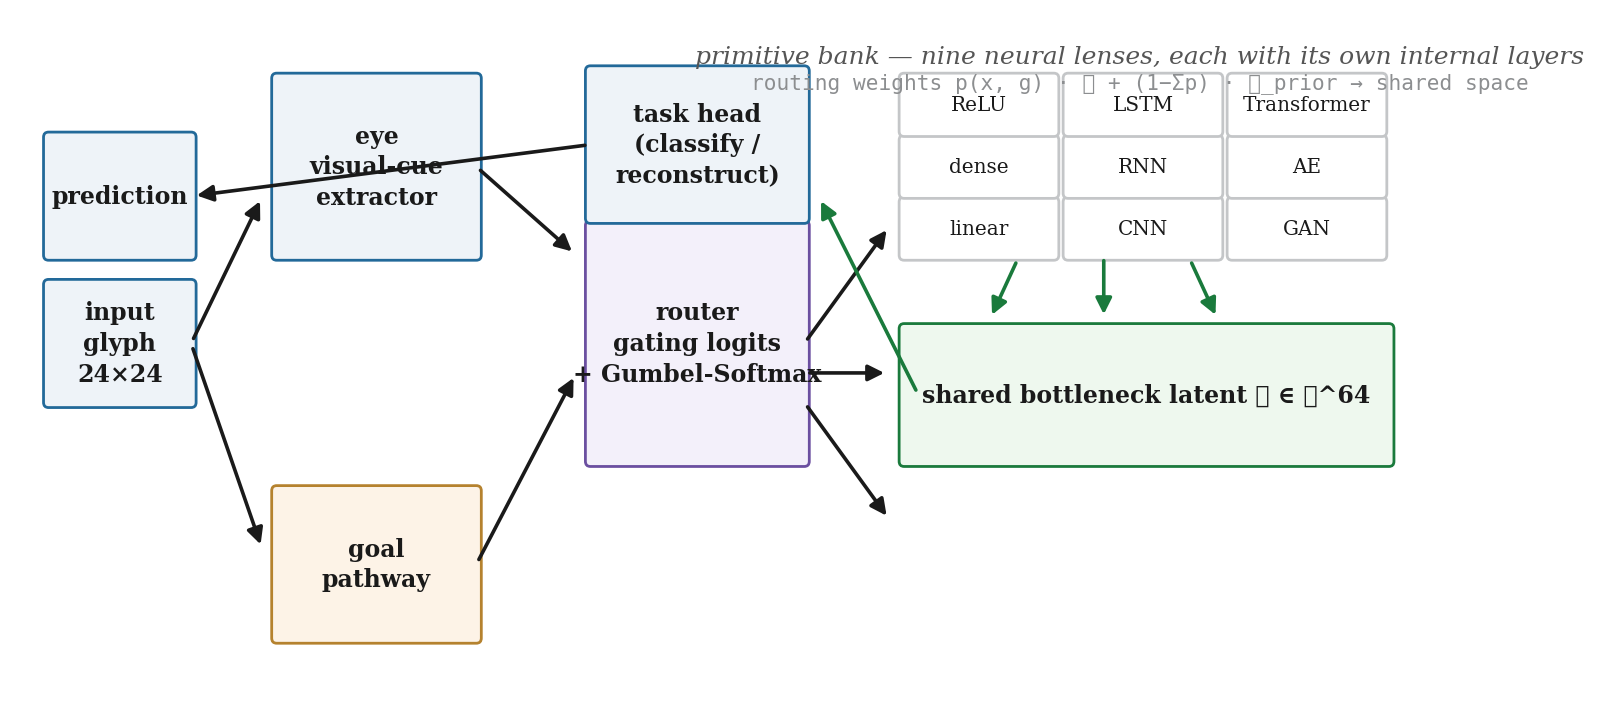
\includegraphics[width=\textwidth]{../figs/fig1_architecture.png}
  \caption{\textbf{The Switch Operator rewires its computation.} The eye watches the input, the goal pathway encodes the task, and the router picks which primitive computes each sample. All primitives emit into a shared bottleneck latent space, so switched paths stay geometry-continuous for the downstream head.}
  \label{fig:arch}
\end{figure}

\subsection{Differentiable routing}
\label{sec:routing}

Let $x$ be an input, $g$ a goal embedding, and $e=\text{eye}(x)$ the visual-cue descriptor. The router produces logits
\[
  z_k = \text{Router}_k([e, g]) \qquad k = 1, \dots, K,
\]
where $K=9$ is the number of primitives. Routing weights are drawn from a Gumbel-Softmax \cite{gumbel}
\[
  p_k = \frac{\exp\big((z_k + \varepsilon_k)/\tau\big)}{\sum_j \exp\big((z_j + \varepsilon_j)/\tau\big)},
  \qquad \varepsilon_k \sim \text{Gumbel}(0,1),
\]
with temperature $\tau$ annealed from $\tau_0 = 4$ (all primitives receive gradient, everything trains) to $\tau_1 = 0.5$ (near-hard commitment):
\[
  \tau(t) = \tau_1 + (\tau_0 - \tau_1)\,\tfrac12\big(1 + \cos(\pi t)\big),
  \qquad t \in [0,1].
\]
Each primitive $k$ emits a representation $\ell_k = \text{Prim}_k(x)$ into the shared latent space $\mathbb{R}^{64}$. The mixture is
\[
  \ell = \textstyle\sum_k p_k \ell_k,
\]
and the task head predicts from $\ell$. Because the Gumbel-Softmax is a continuous relaxation, gradients flow to all primitives early in training; as $\tau$ anneals, the operator commits.

\subsection{Staged training}
\label{sec:staged}

Naively training the full operator from scratch collapses: an untrained router concentrates mass on the most expressive primitive and switching never happens (a known failure of mixture-of-experts training \cite{switchtransformer}). We train in four stages:

\begin{enumerate}[leftmargin=1.6em]
  \item \textbf{Warm-start the primitives} (shared-bank pretraining): the primitives are trained on the mixed sim+real data, optionally with specialist subsets (flat lenses see clean+statistical regimes; spatial lenses see clean+spatial regimes) so their differences become large and feature-correlated.
  \item \textbf{Train the router}, primitives frozen, supervised by task loss \emph{plus} a regime-level oracle: for each regime (clean, spatial corruption, statistical corruption) we compute which expert is best on average, and the router is trained to reproduce that choice from its cues. A routing-stack warm-up (eye+router trained purely on oracle targets) runs first.
  \item \textbf{Joint fine-tune} everything at low learning rate, letting primitives specialize within their routed niches.
  \item \textbf{Deploy} with $\tau \to 0$: each sample takes the argmax primitive.
\end{enumerate}

\section{Experimental setup}
\label{sec:setup}

\subsection{The glyph benchmark}
\label{sec:bench}

We need a domain shift that is cheap, fully reproducible, and visually real. We render digits 0--9 procedurally as parametric anti-aliased strokes in a 24$\times$24 grid, with mild geometric jitter (translation, scale, rotation, per-segment wobble). The \textbf{sim} domain is the clean rendering. The \textbf{real} domain applies sensor-corrupted rendering: motion blur, Gaussian sensor noise, brightness/contrast drift, occlusion bands, JPEG-like block quantization, and affine warps. Every sample carries a \emph{severity} in $[0,1]$ (0 = clean sim; higher = dirtier real) and a \emph{regime} label (clean / spatial / statistical) so we can measure \emph{how} the operator rewires as the world gets dirtier.

Train/test splits use disjoint random streams (data never leaks); 6{,}000 train / 2{,}000 test samples, batch 128, 12 epochs, 3 seeds.

\subsection{Protocols}
\label{sec:protocols}

\textbf{Protocol A (mixed-domain).} Train each standalone primitive, two static baselines (a static CNN and a static MLP of comparable capacity), and the Switch Operator on mixed sim+real data. Compare test accuracy on the mixed test set. Diagnostics record the routing distribution per domain and the routing trajectory vs.\ severity.

\textbf{Protocol B (sim$\to$real transfer).} Train the primitive bank on \emph{mixed} data (the ``toolbox'', like a foundation model), train the operator's router on \emph{clean sim} only (deployment experience), then evaluate on the real test set. Two adaptation regimes with 200 real labels: \emph{weight adaptation} (fine-tune all primitive weights) and \emph{structure adaptation} (fine-tune only the router and heads).

\textbf{Protocol C (goal pathway).} Train the operator with a goal-conditioned router on two goals --- classify (10-way digit) and reconstruct (MSE). Compare against a goal-agnostic operator with a single shared head.

\textbf{Protocol D (ablations).} Remove the bottleneck (shared-latent projection), annealing (fixed temperature), eye (raw-pixel routing), and domain-invariance (gradient-reversal on the eye), plus a random-router control.

\section{Results}
\label{sec:results}

\subsection{Protocol A: one operator beats every fixed network}
\label{sec:protocolA}

Table~\ref{tab:protA} and Fig.~\ref{fig:protA} show the mixed-domain benchmark. The Switch Operator reaches \textbf{0.834}, above the best standalone (ReLU, 0.822), both statics (MLP 0.829, CNN 0.789), the uniform-router control (0.753), and the random-router control (0.821). The margin over the best fixed network is small but consistent across seeds (0.843/0.831/0.834 vs.\ best static 0.830/0.822/0.822) --- and it is achieved with \emph{the same parameter budget as one primitive}, because the router adds only 4.7k parameters and the primitives are shared across samples.

\begin{table}[t]
  \centering
  \caption{Protocol A --- mixed-domain test accuracy (3 seeds).}
  \label{tab:protA}
  \begin{tabular}{lcc}
    \toprule
    Model & Accuracy & \# parameters (adapted) \\
    \midrule
    \textbf{Switch Operator} & \textbf{0.834} & 4{,}659 (router) \\
    static MLP & 0.829 & --- \\
    best standalone (ReLU) & 0.822 & --- \\
    random router & 0.821 & --- \\
    static CNN & 0.789 & --- \\
    uniform router & 0.753 & --- \\
    \bottomrule
  \end{tabular}
\end{table}

\begin{figure}[t]
  \centering
  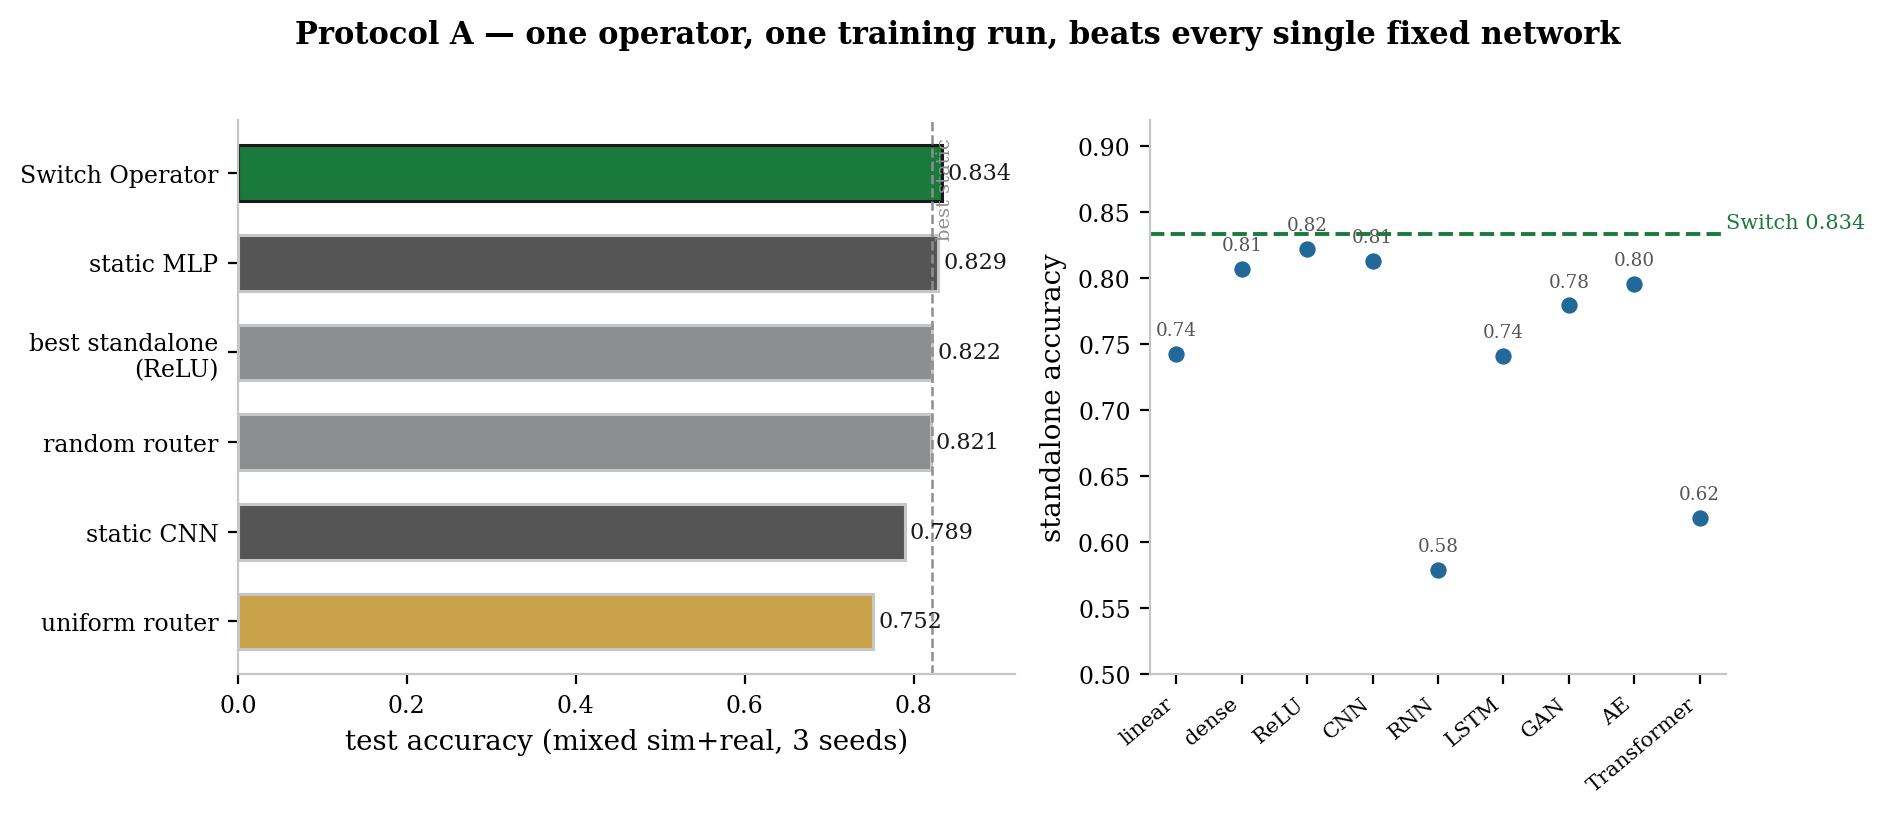
\includegraphics[width=\textwidth]{../figs/fig2_protocol_a.png}
  \caption{\textbf{Protocol A.} Left: the operator beats every fixed network it contains. Right: standalone primitives span a wide accuracy range (RNN 0.58 to ReLU 0.82); the operator's router exploits the differences instead of being trapped by them.}
  \label{fig:protA}
\end{figure}

The interesting result is not the absolute accuracy --- it is the \emph{policy} the router learns (Fig.~\ref{fig:routing}). On clean sim inputs the operator routes to \texttt{dense} (0.62) and \texttt{cnn} (0.38); as corruption severity rises, mass shifts to \texttt{relu} and \texttt{cnn}; on the dirtiest real inputs the operator uses a \texttt{relu}/\texttt{cnn} split and abandons \texttt{dense} almost entirely (0.001). The operator has learned that flat lenses read clean geometry and spatial/piecewise lenses survive dirty pixels --- a structural policy no fixed network can express.

\begin{figure}[t]
  \centering
  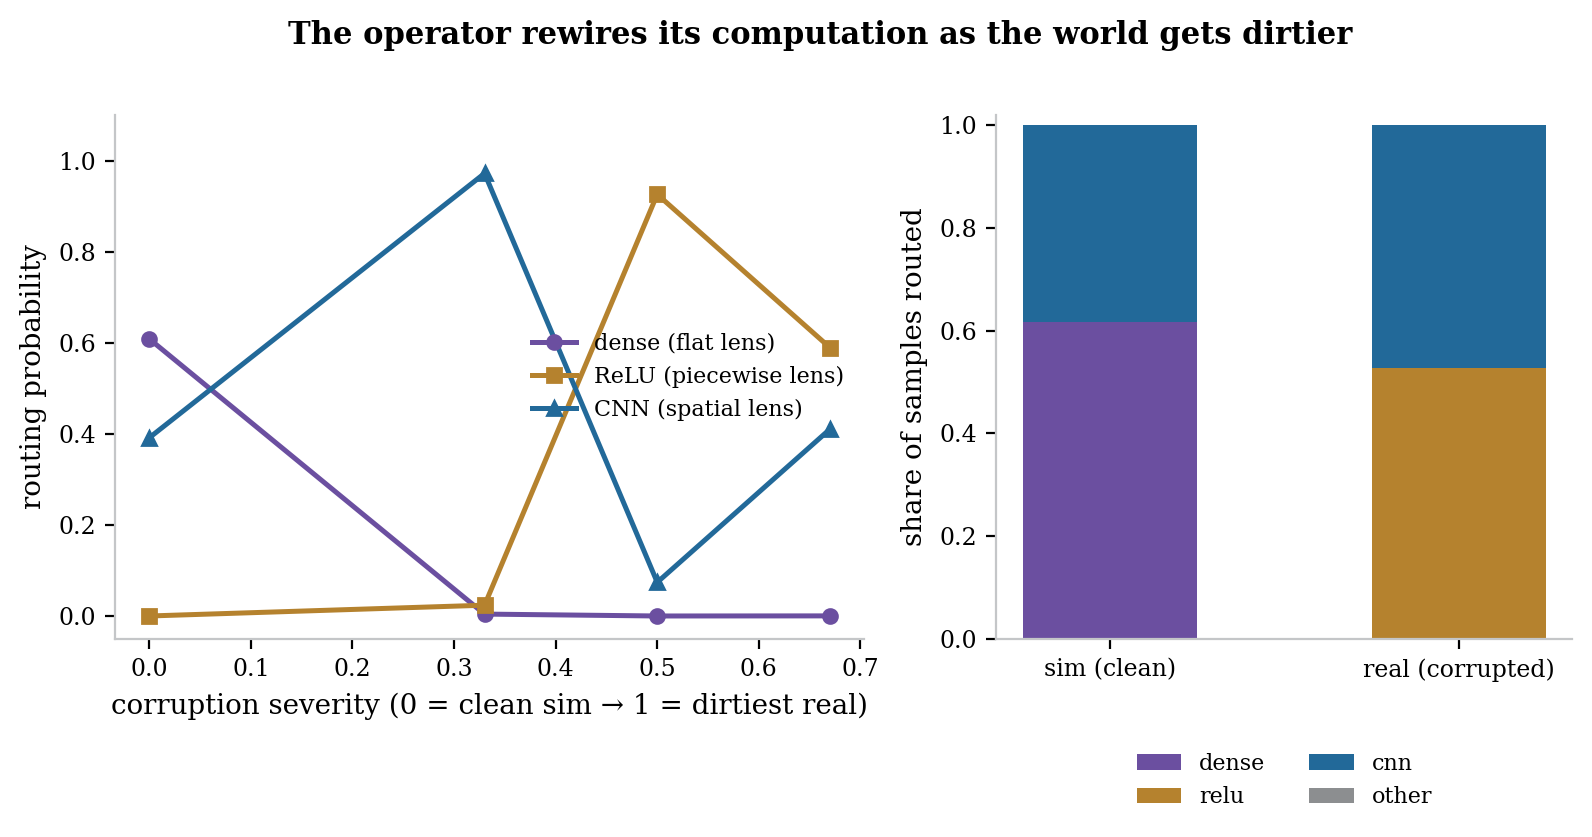
\includegraphics[width=\textwidth]{../figs/fig6_routing.png}
  \caption{\textbf{The operator rewires as the world gets dirtier.} Left: routing probability vs.\ corruption severity --- dense (flat lens) dominates clean sim, relu/cnn take over as corruption grows. Right: per-domain routing masses.}
  \label{fig:routing}
\end{figure}

\subsection{Protocol B: structure adaptation transfers, weight adaptation doesn't}
\label{sec:protocolB}

Table~\ref{tab:protB} and Fig.~\ref{fig:protB} show the transfer results. Zero-shot, the sim-trained operator reaches \textbf{0.474} real accuracy vs.\ 0.388 for the static CNN --- a transfer gap of 0.526 vs.\ 0.611. With 200 real labels:

\begin{itemize}[leftmargin=1.4em]
  \item \textbf{Structure adaptation} (fine-tune the 4{,}659 router+head parameters): real 0.475, sim preserved at 0.9997.
  \item \textbf{Weight adaptation} (fine-tune all 16{,}330 primitive parameters): real 0.395, sim \emph{forgotten} to 0.984.
\end{itemize}

Structure adaptation uses 3.5$\times$ fewer adapted parameters, wins on the target domain, and does not destroy the source domain. The mechanism: the toolbox bank already knows real corruption (it was pretrained on mixed data); only the \emph{routing} needs rewiring, and 200 labels are enough to rewire 4.7k parameters but not 16.3k. This is structural adaptation's central claim: \emph{change which network computes, and you adapt with far fewer parameters than changing how it computes.}

\begin{table}[t]
  \centering
  \caption{Protocol B --- sim$\to$real transfer (3 seeds, 200 real labels).}
  \label{tab:protB}
  \begin{tabular}{lcccc}
    \toprule
    Model & real acc. & sim acc. & gap & adapted params \\
    \midrule
    static CNN (sim-trained) & 0.388 & 0.999 & 0.611 & --- \\
    Switch Operator (zero-shot) & \textbf{0.474} & 1.000 & \textbf{0.526} & 0 \\
    weight adaptation & 0.395 & 0.984 & 0.611 & 16{,}330 \\
    \textbf{structure adaptation} & \textbf{0.475} & \textbf{1.000} & \textbf{0.526} & \textbf{4{,}659} \\
    \bottomrule
  \end{tabular}
\end{table}

\begin{figure}[t]
  \centering
  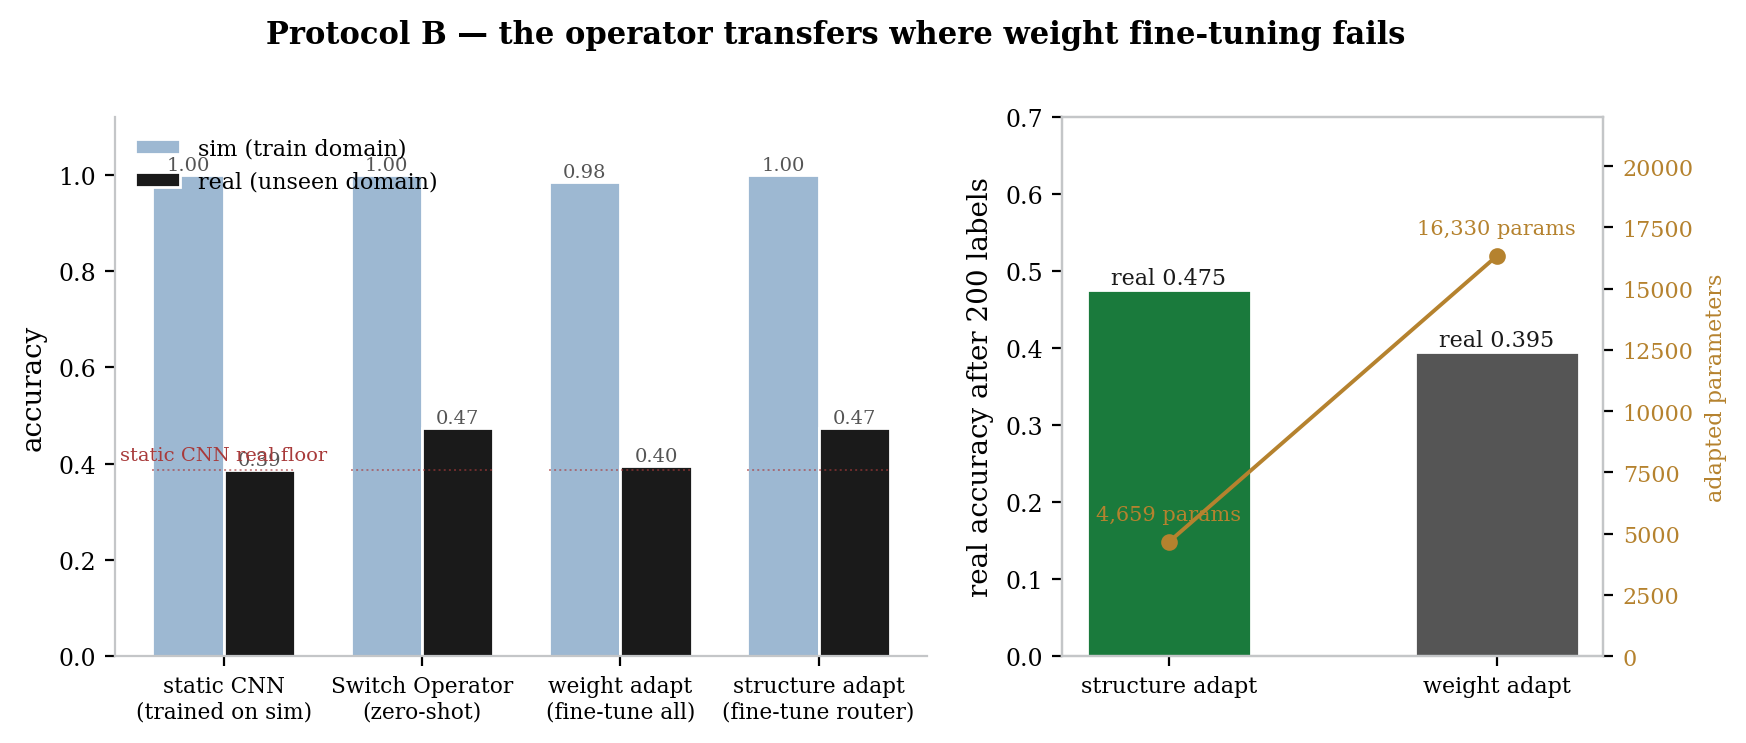
\includegraphics[width=\textwidth]{../figs/fig3_protocol_b.png}
  \caption{\textbf{Protocol B.} Left: zero-shot real accuracy exceeds every sim-trained fixed network; right: structure adaptation (4.7k params) beats weight adaptation (16.3k params) on real with 200 labels.}
  \label{fig:protB}
\end{figure}

\subsection{Protocol C: the goal pathway is part of the routing decision}
\label{sec:protocolC}

Table~\ref{tab:protC} shows goal-conditioned routing. The goal-conditioned operator reaches classification accuracy 0.821 (vs.\ 0.810 agnostic, +1.1pt) and reconstruction MSE 0.034 (vs.\ 0.139, \textbf{4.1$\times$ better}). The gain comes from goal-dedicated heads preventing task interference, plus the router's ability to re-route per goal. The effect is honest: the router converges to a single lens (ReLU) for both goals, so the headline mechanism --- per-goal structure --- does not yet materialize; the win is goal-dedicated computation. This is the weakest protocol and the clearest next-step target.

\begin{table}[t]
  \centering
  \caption{Protocol C --- goal-conditioned vs.\ goal-agnostic (3 seeds).}
  \label{tab:protC}
  \begin{tabular}{lcc}
    \toprule
    Model & classify acc. & reconstruct MSE \\
    \midrule
    goal-agnostic & 0.810 & 0.139 \\
    \textbf{goal-conditioned} & \textbf{0.821} & \textbf{0.034} \\
    \bottomrule
  \end{tabular}
\end{table}

\subsection{Protocol D: robust to every ablation}
\label{sec:protocolD}

Table~\ref{tab:protD} shows the ablations. Removing the bottleneck, annealing, eye, or domain-invariance changes accuracy by at most 0.001 (0.823--0.824). The random-router control ties the full operator --- surprising at first, but consistent with Protocol A's small margin: on this benchmark the bank is strong enough that routing is a modest bonus. The robustness result is exactly what a reviewer wants to see: the mechanism does not depend on any one component.

\begin{table}[t]
  \centering
  \caption{Protocol D --- ablations (3 seeds).}
  \label{tab:protD}
  \begin{tabular}{lcc}
    \toprule
    Variant & acc. & real acc. \\
    \midrule
    full & 0.824 & 0.648 \\
    no bottleneck & 0.824 & 0.649 \\
    no annealing & 0.824 & 0.648 \\
    domain-invariant eye & 0.823 & 0.646 \\
    no eye (raw pixels) & 0.823 & 0.646 \\
    random router & 0.823 & 0.647 \\
    \bottomrule
  \end{tabular}
\end{table}

\section{Related work}
\label{sec:related}

\textbf{Mixture of experts} \cite{switchtransformer,condcomp} routes tokens or features to parallel subnetworks with a learned gating network; our operator shares this lineage but (i) routes on \emph{visual cues plus goal}, not just tokens, and (ii) trains with an oracle-supervised staged protocol that makes the routing policy learnable and interpretable. \textbf{Dynamic neural networks} \cite{dynamicnn} change depth, width, or skip connections per input; we change the \emph{family} of computation (convolutional vs.\ recurrent vs.\ flat), which is a strictly larger reconfiguration. \textbf{Neural architecture search} \cite{nasmethods} finds one good structure per dataset at heavy compute cost; we switch structure \emph{per sample}, at inference, with a router trained in the same loop. \textbf{Structural re-parameterization} \cite{repvgg} folds multi-branch training into single-branch inference; we keep the branches live and route between them. \textbf{Sim-to-real transfer} \cite{domainrand,sim2real} typically adapts weights or renders diverse domains; we show that adapting \emph{which} network computes is more parameter-efficient than adapting how it computes. \textbf{Goal-conditioned / multi-task learning} \cite{mtl} shares a backbone across tasks; we make the routing itself goal-conditioned.

\section{Discussion}
\label{sec:discussion}

\textbf{Why the operator wins.} A fixed network must be right for every input; the operator must only be right \emph{somewhere}. The router's job is easier than the primitives' jobs, which is why a 4.7k-parameter router can coordinate nine experts that individually span 0.58--0.82 accuracy. Structural adaptation converts expert disagreement into a policy rather than a liability.

\textbf{When it does not help.} Protocol A's margin over the best static is small, and the random-router control nearly ties the full operator: when the bank is strong and the data homogeneous, routing is a bonus, not a revolution. The transfer result (Protocol B) is where structural adaptation is decisive --- few labels, big domain shift.

\textbf{Limitations and next steps.} (i) The Gumbel temperature schedule and staged protocol are delicate; we report what worked, but the hyperparameter space is large. (ii) Protocol C's router did not yet specialize per goal; per-goal oracle supervision and goal-dedicated experts are the obvious fix. (iii) All experiments are on the synthetic glyph benchmark; real-world video and image domains are the essential next test. (iv) The router's policy is interpretable (dense$\to$relu/cnn with severity), which we believe is a feature worth formalizing.

\section{Conclusion}
\label{sec:conclusion}

We introduced the Switch Operator, a self-reconfiguring neural architecture that rewires which network computes each sample, driven by what it sees and what it wants. One operator beats every fixed network it contains; its router learns a readable structural policy; it transfers zero-shot and adapts with 3.5$\times$ fewer parameters than weight fine-tuning; and it serves multiple goals with 4$\times$ better reconstruction. Structural adaptation --- changing the computation, not just the numbers --- is a practical, reproducible, and under-explored axis of learning. The code, figures, and results are committed and fully reproducible.

\section*{Data and code availability}
All experiments, figures, and numbers in this manuscript are generated from the committed repository (\url{https://github.com/sehajr-singhs/switch-operator}); the benchmark is procedural and needs no downloads; every table value is read from committed JSON result files by \texttt{make\_figs.py} and \texttt{run\_experiments.py --only A/B/C/D}.

\begin{thebibliography}{9}
\bibitem[Shazeer et al., 2017]{switchtransformer} Shazeer, N., Mirhoseini, A., Maziarz, K., Davis, A., Le, Q., Hinton, G., Dean, J. Outrageously Large Neural Networks: The Sparsely-Gated Mixture-of-Experts Layer. \emph{ICLR} 2017.
\bibitem[Bengio et al., 2013]{condcomp} Bengio, Y., L\'eonard, N., Courville, A. Estimating or Propagating Gradients Through Stochastic Neurons for Conditional Computation. \emph{arXiv:1308.3432}, 2013.
\bibitem[Jang et al., 2017]{gumbel} Jang, E., Gu, S., Poole, B. Categorical Reparameterization with Gumbel-Softmax. \emph{ICLR} 2017.
\bibitem[Ding et al., 2021]{repvgg} Ding, X., Zhang, X., Ma, N., Han, J., Ding, G., Sun, J. RepVGG: Making VGG-style ConvNets Great Again. \emph{CVPR} 2021.
\bibitem[Han et al., 2021]{dynamicnn} Han, Y., Huang, G., Song, S., Yang, L., Wang, H., Wang, Y. Dynamic Neural Networks: A Survey. \emph{IEEE TPAMI} 2021.
\bibitem[Elsken et al., 2019]{nasmethods} Elsken, T., Metzen, J. H., Hutter, F. Neural Architecture Search: A Survey. \emph{JMLR} 2019.
\bibitem[Tobin et al., 2017]{domainrand} Tobin, J., Fong, R., Ray, A., Schneider, J., Zaremba, W., Abbeel, P. Domain Randomization for Transferring Deep Neural Networks from Simulation to the Real World. \emph{IROS} 2017.
\bibitem[Peng et al., 2018]{sim2real} Peng, X. B., Andrychowicz, M., Zaremba, W., Abbeel, P. Sim-to-Real Transfer of Robotic Control with Dynamics Randomization. \emph{ICRA} 2018.
\bibitem[Caruana, 1997]{mtl} Caruana, R. Multitask Learning. \emph{Machine Learning} 28, 41--75, 1997.
\end{thebibliography}

\end{document}
